\documentclass{article}\usepackage[]{graphicx}\usepackage[]{color}
%% maxwidth is the original width if it is less than linewidth
%% otherwise use linewidth (to make sure the graphics do not exceed the margin)
\makeatletter
\def\maxwidth{ %
  \ifdim\Gin@nat@width>\linewidth
    \linewidth
  \else
    \Gin@nat@width
  \fi
}
\makeatother

\definecolor{fgcolor}{rgb}{0.345, 0.345, 0.345}
\newcommand{\hlnum}[1]{\textcolor[rgb]{0.686,0.059,0.569}{#1}}%
\newcommand{\hlstr}[1]{\textcolor[rgb]{0.192,0.494,0.8}{#1}}%
\newcommand{\hlcom}[1]{\textcolor[rgb]{0.678,0.584,0.686}{\textit{#1}}}%
\newcommand{\hlopt}[1]{\textcolor[rgb]{0,0,0}{#1}}%
\newcommand{\hlstd}[1]{\textcolor[rgb]{0.345,0.345,0.345}{#1}}%
\newcommand{\hlkwa}[1]{\textcolor[rgb]{0.161,0.373,0.58}{\textbf{#1}}}%
\newcommand{\hlkwb}[1]{\textcolor[rgb]{0.69,0.353,0.396}{#1}}%
\newcommand{\hlkwc}[1]{\textcolor[rgb]{0.333,0.667,0.333}{#1}}%
\newcommand{\hlkwd}[1]{\textcolor[rgb]{0.737,0.353,0.396}{\textbf{#1}}}%
\let\hlipl\hlkwb

\usepackage{framed}
\makeatletter
\newenvironment{kframe}{%
 \def\at@end@of@kframe{}%
 \ifinner\ifhmode%
  \def\at@end@of@kframe{\end{minipage}}%
  \begin{minipage}{\columnwidth}%
 \fi\fi%
 \def\FrameCommand##1{\hskip\@totalleftmargin \hskip-\fboxsep
 \colorbox{shadecolor}{##1}\hskip-\fboxsep
     % There is no \\@totalrightmargin, so:
     \hskip-\linewidth \hskip-\@totalleftmargin \hskip\columnwidth}%
 \MakeFramed {\advance\hsize-\width
   \@totalleftmargin\z@ \linewidth\hsize
   \@setminipage}}%
 {\par\unskip\endMakeFramed%
 \at@end@of@kframe}
\makeatother

\definecolor{shadecolor}{rgb}{.97, .97, .97}
\definecolor{messagecolor}{rgb}{0, 0, 0}
\definecolor{warningcolor}{rgb}{1, 0, 1}
\definecolor{errorcolor}{rgb}{1, 0, 0}
\newenvironment{knitrout}{}{} % an empty environment to be redefined in TeX

\usepackage{alltt}
\IfFileExists{upquote.sty}{\usepackage{upquote}}{}
\begin{document}

\begin{knitrout}
\definecolor{shadecolor}{rgb}{0.969, 0.969, 0.969}\color{fgcolor}\begin{kframe}
\begin{alltt}
\hlcom{#================================================================}
\hlcom{# graph for hw 2 problem 4}
\hlcom{#}
\hlcom{# Tyler Bradley}
\hlcom{# 1/28/2018}
\hlcom{#================================================================}

\hlcom{# loading required libraries}
\hlkwd{library}\hlstd{(tidyverse)}
\hlkwd{library}\hlstd{(knitr)}
\hlkwd{library}\hlstd{(kableExtra)}
\end{alltt}
\end{kframe}
\end{knitrout}

Part a
Defining constants

\begin{knitrout}
\definecolor{shadecolor}{rgb}{0.969, 0.969, 0.969}\color{fgcolor}\begin{kframe}
\begin{alltt}
\hlstd{a} \hlkwb{<-} \hlnum{4}
\hlstd{b} \hlkwb{<-} \hlnum{1}
\hlstd{k} \hlkwb{<-} \hlnum{1054.08} \hlcom{# [=] $M^\{-1\} * days^\{-1\}$}
\hlstd{cb_o} \hlkwb{=} \hlnum{6.25e-5} \hlcom{# [=] M}
\hlstd{ca_o} \hlkwb{=} \hlnum{9.101e-6} \hlcom{# [=] M}
\end{alltt}
\end{kframe}
\end{knitrout}

Creating data set
$C_{Mn}$ is calculated from formula derived in problem

\begin{knitrout}
\definecolor{shadecolor}{rgb}{0.969, 0.969, 0.969}\color{fgcolor}\begin{kframe}
\begin{alltt}
\hlstd{mn_data} \hlkwb{<-} \hlkwd{tibble}\hlstd{(}\hlkwc{t_days} \hlstd{=} \hlkwd{seq}\hlstd{(}\hlnum{0}\hlstd{,} \hlnum{60}\hlstd{,} \hlkwc{by} \hlstd{=} \hlnum{1}\hlstd{))} \hlopt
  \hlkwd{mutate}\hlstd{(}\hlkwc{c_mn_mol} \hlstd{= ((ca_o} \hlopt{-} \hlstd{(a} \hlopt{/} \hlstd{b)} \hlopt{*} \hlstd{cb_o)} \hlopt{/} \hlstd{(}
    \hlnum{1} \hlopt{-} \hlstd{(a} \hlopt{/} \hlstd{b)} \hlopt{*} \hlstd{(cb_o} \hlopt{/} \hlstd{ca_o)} \hlopt{*} \hlkwd{exp}\hlstd{(}\hlopt{-}\hlstd{(((}
      \hlstd{b} \hlopt{*} \hlstd{ca_o}
    \hlstd{)} \hlopt{/} \hlstd{(}
      \hlstd{a} \hlopt{*} \hlstd{cb_o}
    \hlstd{))} \hlopt{-} \hlnum{1}\hlstd{)} \hlopt{*} \hlstd{cb_o} \hlopt{*} \hlstd{k} \hlopt{*} \hlstd{t_days)}
  \hlstd{)),}
  \hlkwc{c_mn_ug} \hlstd{= c_mn_mol} \hlopt{*} \hlnum{54.938} \hlopt{*} \hlnum{1e6}\hlstd{)}
\end{alltt}
\end{kframe}
\end{knitrout}

Plotting the decay equation

\begin{knitrout}
\definecolor{shadecolor}{rgb}{0.969, 0.969, 0.969}\color{fgcolor}\begin{kframe}
\begin{alltt}
\hlkwd{ggplot}\hlstd{(mn_data,} \hlkwd{aes}\hlstd{(t_days, c_mn_ug))} \hlopt{+}
  \hlkwd{geom_point}\hlstd{()} \hlopt{+}
  \hlkwd{geom_line}\hlstd{()} \hlopt{+}
  \hlkwd{theme_bw}\hlstd{()} \hlopt{+}
  \hlkwd{scale_y_continuous}\hlstd{(}\hlkwc{breaks} \hlstd{=} \hlkwd{seq}\hlstd{(}\hlnum{0}\hlstd{,} \hlnum{500}\hlstd{,} \hlkwc{by} \hlstd{=} \hlnum{20}\hlstd{))}
\end{alltt}
\end{kframe}
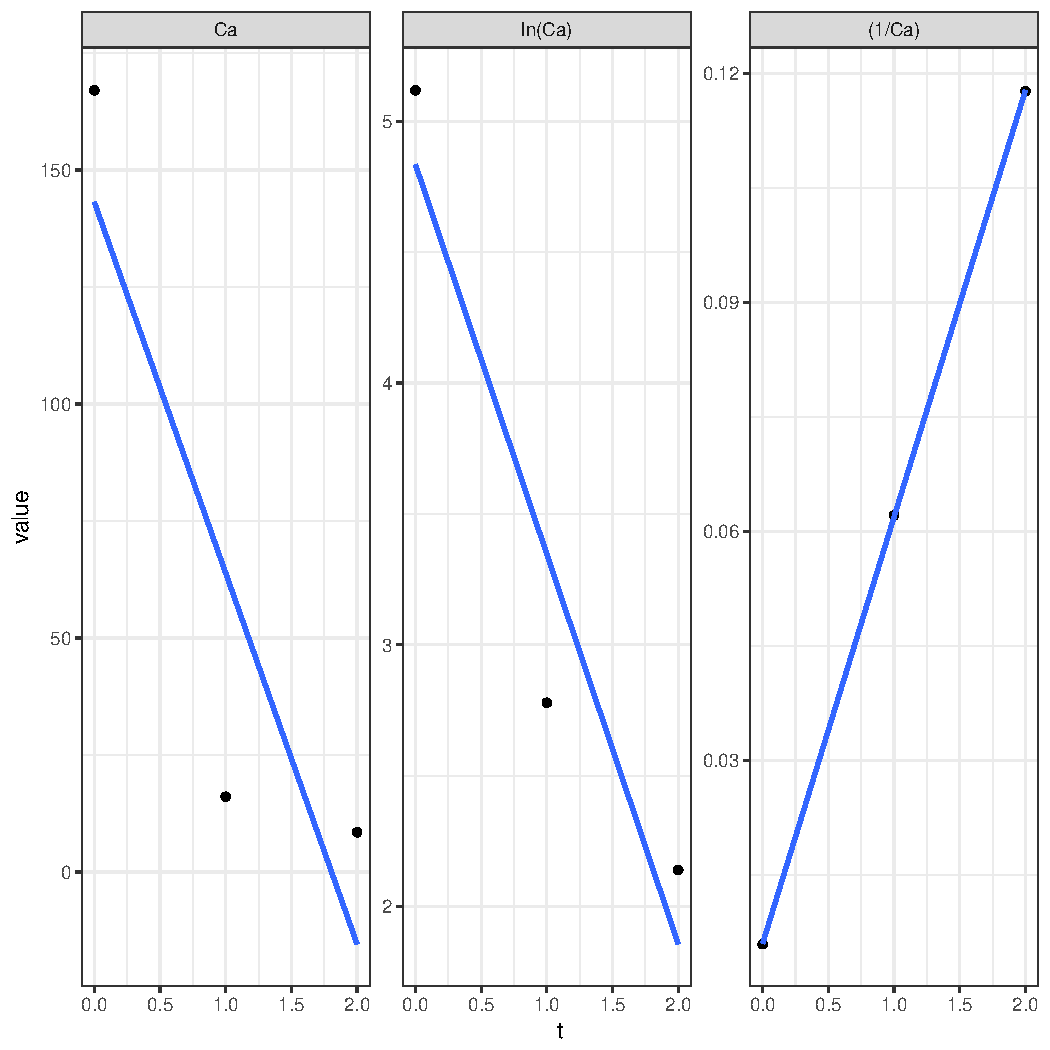
\includegraphics[width=\maxwidth]{figure/unnamed-chunk-4-1} 

\end{knitrout}

Part b
$CO_{2}$ is in great excess so $r_{mn}$ becomes a psuedo-first order equation

\begin{knitrout}
\definecolor{shadecolor}{rgb}{0.969, 0.969, 0.969}\color{fgcolor}\begin{kframe}
\begin{alltt}
\hlstd{k_star} \hlkwb{<-} \hlstd{k} \hlopt{*} \hlstd{cb_o}

\hlstd{mn_data_b} \hlkwb{<-} \hlkwd{tibble}\hlstd{(}\hlkwc{t_days} \hlstd{=} \hlkwd{seq}\hlstd{(}\hlnum{0}\hlstd{,} \hlnum{60}\hlstd{,} \hlkwc{by} \hlstd{=} \hlnum{1}\hlstd{))} \hlopt
  \hlkwd{mutate}\hlstd{(}\hlkwc{c_mn_mol} \hlstd{= ca_o} \hlopt{*} \hlkwd{exp}\hlstd{(}\hlopt{-}\hlstd{k_star}\hlopt{*}\hlstd{t_days),}
         \hlkwc{c_mn_ug} \hlstd{= c_mn_mol} \hlopt{*} \hlnum{54.938} \hlopt{*} \hlnum{1e6}\hlstd{)}
\end{alltt}
\end{kframe}
\end{knitrout}

Plotting decay rxn as psuedo-first order

\begin{knitrout}
\definecolor{shadecolor}{rgb}{0.969, 0.969, 0.969}\color{fgcolor}\begin{kframe}
\begin{alltt}
\hlkwd{ggplot}\hlstd{(mn_data_b,} \hlkwd{aes}\hlstd{(t_days, c_mn_ug))} \hlopt{+}
  \hlkwd{geom_point}\hlstd{()} \hlopt{+}
  \hlkwd{geom_line}\hlstd{()} \hlopt{+}
  \hlkwd{theme_bw}\hlstd{()} \hlopt{+}
  \hlkwd{scale_y_continuous}\hlstd{(}\hlkwc{breaks} \hlstd{=} \hlkwd{seq}\hlstd{(}\hlnum{0}\hlstd{,} \hlnum{500}\hlstd{,} \hlkwc{by} \hlstd{=} \hlnum{20}\hlstd{))}
\end{alltt}
\end{kframe}
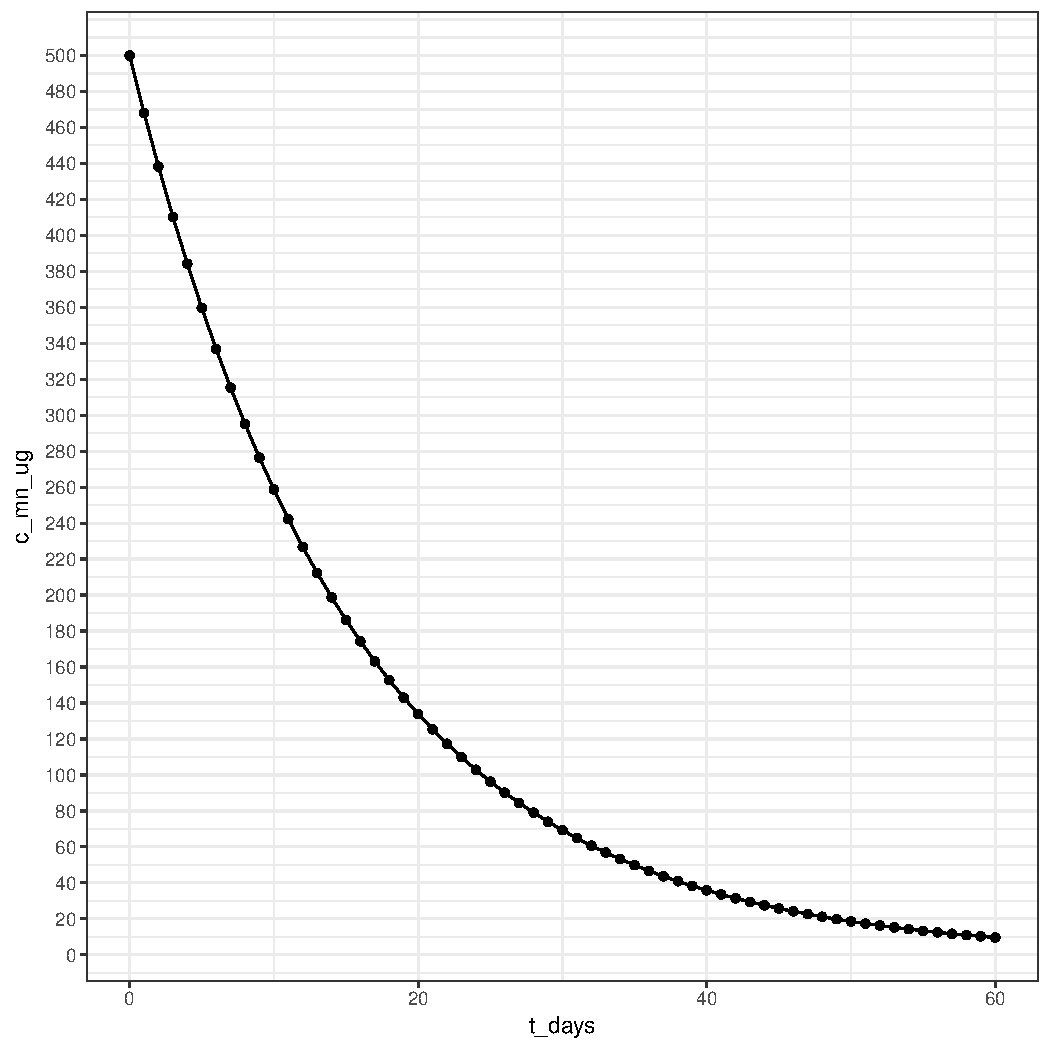
\includegraphics[width=\maxwidth]{figure/unnamed-chunk-6-1} 

\end{knitrout}

\end{document}
